\chapter{Planar Graphs}

\tikzset{vtx/.style={circle,fill=black,inner sep=1.6pt}}

\section{Planar embeddings and faces}

\begin{definition}[Planar]
A graph is \emph{planar} if it can be drawn in the plane so that edges meet only at common
ends (no crossings). Such a drawing is a \emph{planar embedding}.
\end{definition}

$K_4$ is planar even though its usual drawing (a square with both diagonals) has a crossing:
move one diagonal outside the square.

\begin{center}
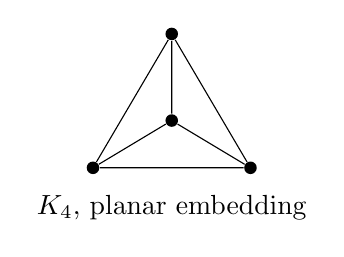
\begin{tikzpicture}
  \node[vtx] (a) at (0,0) {};
  \node[vtx] (b) at (2,0) {};
  \node[vtx] (c) at (1,1.7) {};
  \node[vtx] (d) at (1,0.6) {};
  \draw (a)--(b)--(c)--(a) (a)--(d) (b)--(d) (c)--(d);
  \node at (1,-0.5) {$K_4$, planar embedding};
\end{tikzpicture}
\end{center}

\begin{definition}[Face]
A planar embedding divides the plane into connected regions called \emph{faces}; exactly one
face is unbounded (the \emph{outer} face). Two faces are \emph{adjacent} if they share an edge.
The \emph{boundary walk} of a face is the closed walk around its boundary, and the
\emph{degree} of a face $f$, $\deg(f)$, is the length of its boundary walk.
\end{definition}

A bridge is traversed twice by the boundary walk of the (single) face on both of its sides, so
it contributes $2$ to that face's degree. For example a tree has one face, of degree
$2(p-1)$. The embedding of $K_4$ above has $4$ faces, each of degree $3$.

\begin{example}
The embedding below has $p = 6$ vertices, $q = 7$ edges and $3$ faces. The bridge $cd$ lies inside
the outer face $f_3$, whose boundary walk $a\,b\,c\,d\,e\,d\,c\,f\,a$ traverses it twice, so
$\deg(f_3) = 8$ (counting $de$ twice as well). With $\deg(f_1) = 3$ and $\deg(f_2) = 3$:
$3 + 3 + 8 = 14 = 2q$.
\begin{center}
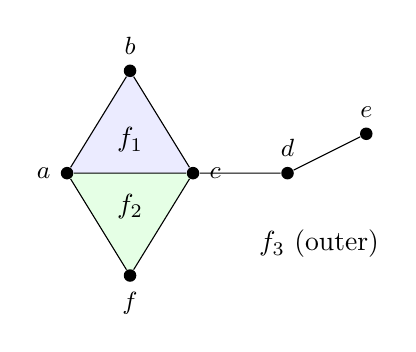
\begin{tikzpicture}[every label/.style={font=\small}]
  \fill[blue!8] (0,0) -- (1.6,0) -- (0.8,1.3) -- cycle;
  \fill[green!10] (0,0) -- (1.6,0) -- (0.8,-1.3) -- cycle;
  \node[vtx,label=left:$a$] (a) at (0,0) {};
  \node[vtx,label=above:$b$] (b) at (0.8,1.3) {};
  \node[vtx,label=right:$c$] (c) at (1.6,0) {};
  \node[vtx,label=below:$f$] (f) at (0.8,-1.3) {};
  \node[vtx,label=above:$d$] (d) at (2.8,0) {};
  \node[vtx,label=above:$e$] (e) at (3.8,0.5) {};
  \draw (a)--(b)--(c)--(f)--(a)--(c) (c)--(d)--(e);
  \node at (0.8,0.42) {$f_1$};
  \node at (0.8,-0.42) {$f_2$};
  \node at (3.2,-0.9) {$f_3$ (outer)};
\end{tikzpicture}
\end{center}
\end{example}

\begin{theorem}[Faceshaking lemma]
For a planar embedding of $G$ with face set $F$, $\displaystyle\sum_{f\in F}\deg(f) = 2\abs{E(G)}$.
\end{theorem}
\begin{proof}
Each edge is traversed exactly twice in total by the boundary walks: once for each side (both
times by the same face if it is a bridge, otherwise once by each of the two different faces on
its two sides).
\end{proof}

\section{Euler's formula}

\begin{theorem}[Euler's formula]
If $G$ is a connected planar graph with $p$ vertices and $q$ edges, then any planar embedding of
$G$ has exactly $f = q - p + 2$ faces; that is, $p - q + f = 2$.
\end{theorem}
\begin{proof}
Induction on $q$. Since $G$ is connected, $q \ge p - 1$. If $q = p - 1$, $G$ is a tree, which has
one face, and $p - (p-1) + 1 = 2$. If $q \ge p$, $G$ is not a tree, so it has a cycle; let $e$ be
an edge of a cycle. Then $e$ is not a bridge, so $G - e$ is connected, and the two faces on either
side of $e$ are distinct (by the Jordan curve theorem the cycle separates the plane) and merge into
one when $e$ is removed. So $G - e$ has $p$ vertices, $q - 1$ edges and $f - 1$ faces, and by
induction $p - (q-1) + (f-1) = 2$, i.e.\ $p - q + f = 2$.
\end{proof}

\begin{corollary}
A planar graph with $p$ vertices, $q$ edges and $c$ components has $f = q - p + 1 + c$ faces in
any planar embedding.
\end{corollary}

In particular the number of faces does not depend on the embedding.

\section{Edge bounds and non-planar graphs}

\begin{lemma}
If $G$ is a planar embedding containing a cycle, then the boundary of each face contains a cycle,
so each face has degree at least the girth of $G$.
\end{lemma}

\begin{theorem}
Let $G$ be a planar graph with $p \ge 3$ vertices and $q$ edges. Then $q \le 3p - 6$.
\end{theorem}
\begin{proof}
It suffices to prove this for connected $G$ (adding edges between components keeps a graph
planar). If $G$ is a tree, $q = p - 1 \le 3p - 6$ since $p \ge 3$ (so $p-1 \le 3p-6 \iff p\ge 2.5$).
Otherwise every face has degree at least $3$, so by faceshaking $2q = \sum\deg(f) \ge 3f$. Using
Euler, $f = q - p + 2$, so $2q \ge 3(q - p + 2)$, i.e.\ $q \le 3p - 6$.
\end{proof}

\begin{corollary}
$K_5$ is not planar.
\end{corollary}
\begin{proof}
$K_5$ has $p = 5$ and $q = 10 > 3\cdot5 - 6 = 9$.
\end{proof}

\begin{theorem}
Let $G$ be a planar graph with $p \ge 3$ vertices, $q$ edges and no $3$-cycles (for example, any
bipartite graph). Then $q \le 2p - 4$.
\end{theorem}
\begin{proof}
As before we may assume $G$ is connected and not a tree (trees satisfy $p - 1 \le 2p - 4$ for
$p\ge3$). Then every face boundary contains a cycle of length at least $4$, so $\deg(f)\ge 4$ and
$2q \ge 4f = 4(q - p + 2)$, giving $q \le 2p - 4$.
\end{proof}

\begin{corollary}
$K_{3,3}$ is not planar.
\end{corollary}
\begin{proof}
$K_{3,3}$ is bipartite, so has no odd cycles, with $p = 6$ and $q = 9 > 2\cdot6-4 = 8$.
\end{proof}

\begin{important}[Pitfall]
The inequalities $q \le 3p-6$ and $q\le 2p-4$ are \emph{necessary} conditions only. A graph
satisfying them may still be non-planar (e.g.\ $K_{3,3}$ satisfies $q \le 3p-6$; the Petersen graph,
with $p = 10$ and $q = 15$, satisfies both, yet is non-planar).
\end{important}

\begin{corollary}
Every planar graph has a vertex of degree at most $5$.
\end{corollary}
\begin{proof}
If $p \le 2$ this is clear. Otherwise $\sum\deg(v) = 2q \le 6p - 12$, so the average degree is at
most $6 - 12/p < 6$, and some vertex has degree at most the average, hence at most $5$.
\end{proof}

\section{Kuratowski's theorem}

\begin{definition}[Edge subdivision]
A \emph{subdivision} of $G$ is a graph obtained by replacing edges of $G$ with paths (inserting
new degree-$2$ vertices along edges).
\end{definition}

A subdivision of $G$ is planar iff $G$ is. Since every subgraph of a planar graph is planar, a
graph containing a subdivision of $K_5$ or $K_{3,3}$ as a subgraph is not planar. Remarkably the
converse holds.

\begin{theorem}[Kuratowski]
A graph is planar if and only if it does not contain a subdivision of $K_5$ or of $K_{3,3}$ as a
subgraph.
\end{theorem}

We do not prove the hard direction. In practice: to show a graph is planar, draw it; to show it is
not, find a subdivision of $K_5$ or $K_{3,3}$ inside it (or use an edge bound).

\begin{center}
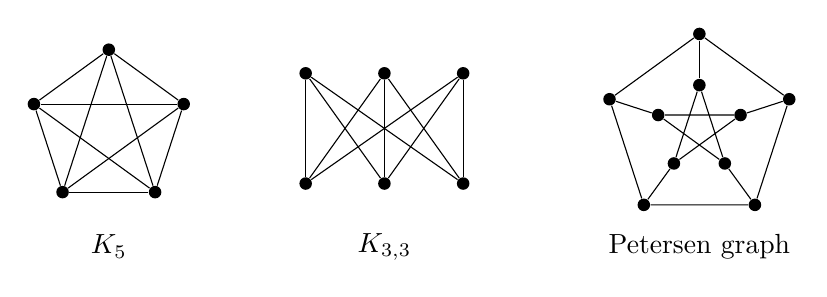
\begin{tikzpicture}
  \foreach \i in {1,...,5} \node[vtx] (k\i) at ({72*\i+18}:1) {};
  \foreach \i in {1,...,5} \foreach \j in {1,...,5} { \ifnum\i<\j \draw (k\i)--(k\j); \fi }
  \node at (0,-1.5) {$K_5$};
  \begin{scope}[xshift=3.5cm,yshift=-0.7cm]
  \foreach \i in {1,2,3} { \node[vtx] (x\i) at (\i-2,1.4) {}; \node[vtx] (y\i) at (\i-2,0) {}; }
  \foreach \i in {1,2,3} \foreach \j in {1,2,3} \draw (x\i)--(y\j);
  \node at (0,-0.8) {$K_{3,3}$};
  \end{scope}
  \begin{scope}[xshift=7.5cm]
  \foreach \i in {1,...,5} {
    \node[vtx] (o\i) at ({72*\i+18}:1.2) {};
    \node[vtx] (n\i) at ({72*\i+18}:0.55) {};
    \draw (o\i)--(n\i);
  }
  \draw (o1)--(o2)--(o3)--(o4)--(o5)--(o1);
  \draw (n1)--(n3)--(n5)--(n2)--(n4)--(n1);
  \node at (0,-1.5) {Petersen graph};
  \end{scope}
\end{tikzpicture}
\end{center}

\begin{example}
The Petersen graph is not planar: it has girth $5$, so a planar embedding would need
$2q \ge 5f$, i.e.\ $30 \ge 5(15 - 10 + 2) = 35$, a contradiction. (It also contains a subdivision
of $K_{3,3}$.)
\end{example}

\section{Platonic solids}

A \emph{platonic graph} is a planar embedding in which every vertex has degree $d \ge 3$ and every
face has degree $d^* \ge 3$. These correspond to the regular polyhedra.

\begin{theorem}
If a connected planar embedding has all vertices of degree $d\ge3$ and all faces of degree
$d^*\ge3$, then $(d,d^*)$ is one of $(3,3), (3,4), (4,3), (3,5), (5,3)$.
\end{theorem}
\begin{proof}
By the handshake and faceshaking lemmas, $dp = 2q$ and $d^*f = 2q$, so $p = 2q/d$ and $f = 2q/d^*$.
Euler's formula gives
\[
\frac{2q}{d} - q + \frac{2q}{d^*} = 2
\quad\Longrightarrow\quad
q\,(2d^* - dd^* + 2d) = 2dd^*.
\]
Since $q, d, d^* > 0$ we need $2d + 2d^* - dd^* > 0$, i.e.\ $(d-2)(d^*-2) < 4$. With $a = d-2\ge1$
and $b = d^*-2 \ge 1$, the positive integer solutions of $ab < 4$ are
$(a,b) \in \{(1,1),(1,2),(2,1),(1,3),(3,1)\}$, giving the five pairs listed.
\end{proof}

Solving $q = \frac{2dd^*}{2d+2d^*-dd^*}$ and then $p = 2q/d$, $f = 2q/d^*$:

\begin{center}
\begin{tabular}{ccccccl}
\toprule
$d$ & $d^*$ & $2d + 2d^* - dd^*$ & $q$ & $p$ & $f$ & solid \\
\midrule
$3$ & $3$ & $3$ & $6$ & $4$ & $4$ & tetrahedron ($K_4$)\\
$3$ & $4$ & $2$ & $12$ & $8$ & $6$ & cube ($Q_3$)\\
$4$ & $3$ & $2$ & $12$ & $6$ & $8$ & octahedron\\
$3$ & $5$ & $1$ & $30$ & $20$ & $12$ & dodecahedron\\
$5$ & $3$ & $1$ & $30$ & $12$ & $20$ & icosahedron\\
\bottomrule
\end{tabular}
\end{center}

For example, for $(3,5)$: $q = \frac{2\cdot15}{6 + 10 - 15} = 30$, $p = 60/3 = 20$, $f = 60/5 = 12$.

The cube and the octahedron as planar embeddings (flatten the solid through one face, which
becomes the outer face):
\begin{center}
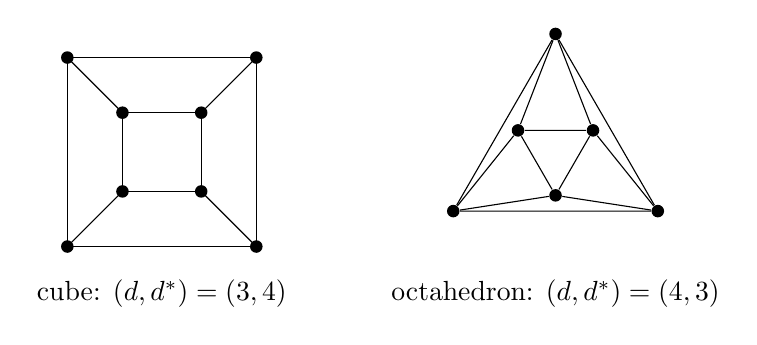
\begin{tikzpicture}
  \draw (-1.2,-1.2) rectangle (1.2,1.2) (-0.5,-0.5) rectangle (0.5,0.5);
  \foreach \x/\y in {-1.2/-1.2,1.2/-1.2,1.2/1.2,-1.2/1.2} {
    \node[vtx] at (\x,\y) {}; \node[vtx] at (\x*0.4167,\y*0.4167) {};
    \draw (\x,\y) -- (\x*0.4167,\y*0.4167);
  }
  \node at (0,-1.8) {cube: $(d,d^*) = (3,4)$};
  \begin{scope}[xshift=5cm]
    \foreach \i in {1,2,3} {
      \node[vtx] (o\i) at ({90+120*\i}:1.5) {};
      \node[vtx] (n\i) at ({30+120*\i}:0.55) {};
    }
    \draw (o1)--(o2)--(o3)--(o1) (n1)--(n2)--(n3)--(n1);
    \draw (o1)--(n1) (o1)--(n2) (o2)--(n2) (o2)--(n3) (o3)--(n3) (o3)--(n1);
    \node at (0,-1.8) {octahedron: $(d,d^*) = (4,3)$};
  \end{scope}
\end{tikzpicture}
\end{center}

\section{Colouring planar graphs}

A \emph{$k$-colouring} assigns one of $k$ colours to each vertex so that adjacent vertices get
different colours (see the next chapter for more). $K_n$ needs $n$ colours, so planar graphs can
need $4$ ($K_4$). How many are always enough?

\begin{theorem}[Six colour theorem]
Every planar graph is $6$-colourable.
\end{theorem}
\begin{proof}
Induction on $p$. For $p = 1$ it is trivial. Otherwise pick a vertex $v$ of degree at most $5$.
$G - v$ is planar, so by induction it has a $6$-colouring. The neighbours of $v$ use at most $5$
colours, so one of the six colours is free for $v$.
\end{proof}

\begin{theorem}[Five colour theorem]
Every planar graph is $5$-colourable.
\end{theorem}
\begin{proof}
Induction on $p$; the cases $p\le5$ are trivial. Let $v$ be a vertex of degree at most $5$. If
$\deg(v) \le 4$, colour $G - v$ by induction and give $v$ a colour not used on its at most $4$
neighbours.

Suppose $\deg(v) = 5$. Since $K_5$ is not planar, two neighbours $x, y$ of $v$ are not adjacent.
Form $G'$ from $G$ by contracting the edges $vx$ and $vy$: merge $x, v, y$ into a single new
vertex $z$ adjacent to every neighbour of $x$, $v$ or $y$ (removing duplicate edges). Contracting
an edge of a planar graph gives a planar graph, so $G'$ is planar with $p - 2$ vertices, and by
induction has a $5$-colouring.
\begin{center}
\begin{tikzpicture}[>={Stealth},every label/.style={font=\small}]
  \node[vtx,fill=white,draw,label=below:$v$] (v) at (0,0) {};
  \foreach \i/\l in {1/x,2/{},3/y,4/{},5/{}} {
    \node[vtx,label={[font=\small]{90+72*(\i-1)}:$\l$}] (u\i) at ({90+72*(\i-1)}:1.2) {};
    \draw (v)--(u\i);
  }
  \draw (u1)--(u2) (u3)--(u4)--(u5)--(u1);
  \draw[->,thick] (2,0) -- node[above,font=\scriptsize] {contract $vx$, $vy$} (3.6,0);
  \begin{scope}[xshift=5.6cm]
    \node[vtx,fill=red!70!black,label=below:$z$] (z) at (0,0) {};
    \foreach \i in {2,4,5} { \node[vtx] (w\i) at ({90+72*(\i-1)}:1.2) {}; \draw (z)--(w\i); }
    \draw (w4)--(w5);
  \end{scope}
\end{tikzpicture}
\end{center}
(Left: $v$ with its five neighbours, $x$ and $y$ non-adjacent. Right: $x$, $v$, $y$ merged into
$z$; afterwards $x$ and $y$ both receive the colour of $z$.)
 Colour $G$ by giving $x$ and $y$ the colour of $z$ and every other
vertex except $v$ its colour in $G'$. This is a proper colouring of $G - v$: $x$ and $y$ are not
adjacent, and any neighbour of $x$ or $y$ was a neighbour of $z$. Now the five neighbours of $v$
use at most $4$ colours (since $x, y$ share one), leaving a colour for $v$.
\end{proof}

\begin{theorem}[Four colour theorem; Appel--Haken 1976]
Every planar graph is $4$-colourable.
\end{theorem}

The proof reduces the problem to checking a large but finite set of configurations by computer;
there is no known short proof.

\section{Summary}
\begin{itemize}
  \item Faceshaking: $\sum\deg(f) = 2q$. Euler: $p - q + f = 2$ for connected planar graphs.
  \item Planar, $p\ge3$: $q \le 3p - 6$; with no triangles: $q\le 2p-4$. Hence $K_5$, $K_{3,3}$
        non-planar.
  \item Kuratowski: planar iff no subdivision of $K_5$ or $K_{3,3}$.
  \item Exactly five platonic solids.
  \item Planar graphs have a vertex of degree $\le 5$; they are $6$-, $5$- and in fact $4$-colourable.
\end{itemize}
